\documentclass[twoside]{article}

\usepackage{aistats2020}
% If your paper is accepted, change the options for the package
% aistats2020 as follows:
%
% \usepackage[accepted]{aistats2020}
%
% This option will print headings for the title of your paper and
% headings for the authors names, plus a copyright note at the end of
% the first column of the first page.

% If you set papersize explicitly, activate the following three lines:
%\special{papersize = 8.5in, 11in}
%\setlength{\pdfpageheight}{11in}
%\setlength{\pdfpagewidth}{8.5in}

% If you use natbib package, activate the following three lines:
%\usepackage[round]{natbib}
%\renewcommand{\bibname}{References}
%\renewcommand{\bibsection}{\subsubsection*{\bibname}}

% If you use BibTeX in apalike style, activate the following line:
%\bibliographystyle{apalike}

\input{math_commands.tex}

\begin{document}

% If your paper is accepted and the title of your paper is very long,
% the style will print as headings an error message. Use the following
% command to supply a shorter title of your paper so that it can be
% used as headings.
%
%\runningtitle{I use this title instead because the last one was very long}

% If your paper is accepted and the number of authors is large, the
% style will print as headings an error message. Use the following
% command to supply a shorter version of the authors names so that
% they can be used as headings (for example, use only the surnames)
%
%\runningauthor{Surname 1, Surname 2, Surname 3, ...., Surname n}

\twocolumn[

\aistatstitle{Provable Online Learning and Bandit Algorithms with Neural Networks}

\aistatsauthor{ Author 1 \And Author 2 \And  Author 3 }

\aistatsaddress{ Institution 1 \And  Institution 2 \And Institution 3 } ]

\begin{abstract}
Problem: contextual bandit

nnet: generalization across $\rvs, \rva$

theoretically justified
\end{abstract}

\input{introduction.tex}

\input{background.tex}

\section{Online Learning with Non-Convex Objectives and Dynamic Regret}
\label{sec:online_learning}

Online learning has been well studied through online convex optimization \citep{shalev2012online}. We consider different assumptions of non-convex, smooth, gradient dominant functions, which are suitable for our problems and algorithms.

\begin{asmp}[Bounded and smooth]
\label{asmp:boundedness_smoothness}
$\left| f_t(\rvx) \right| \le 1$, $\left\| \nabla f_t(\rvx ) - \nabla f_t(\rvy) \right\| \le L $, $\forall \rvx, \rvy$, $\forall t$.
\end{asmp}

\begin{asmp}[Gradient dominant]
\label{asmp:gradient_dominant}
$\left\| \nabla f_t(\rvx) \right\| \ge G \left[ f_t(\rvx) - \min_{\rvw}{ f_t(\rvw )} \right]$, $\forall \rvx$, $\forall t$.
\end{asmp}

\begin{defi}[Functional variation \citep{besbes2015non}]
\label{defi:function_variation}
$V_{T}^{f} \coloneqq \sum_{t=0}^{T-1}{\max\limits_{\rvw}{\left| f_{t+1}(\rvw) - f_{t}(\rvw) \right| } }.$
\end{defi}

Given a sequence of functions $\left\{ f_t : t = 0, 1, \dots, T \right\}$, $V_{T}^{f} $ characterizes how fast/slowly $f_t$ changes over time. For a fast changing sequence with large $V_{T}^{f} $, it is difficult to learn/optimize $f_t$, which is known in online convex optimization literature \citep{jadbabaie2015online}. Under non-convex assumptions, we establish the following result for online gradient update.

\begin{thm}
\label{thm:online_learning_regret}
For any sequence of functions $\left\{ f_t : t = 0, 1, \dots, T \right\}$ that satisfies \cref{asmp:boundedness_smoothness} and \cref{asmp:gradient_dominant}, dynamic regret of online gradient update $\rvx_{t+1} \gets \rvx_{t} - \eta \nabla f_{t}(\rvx_{t})$ with $\eta = 1/L$ satisfies,
\begin{equation}
\label{eq:online_learning_regret}
\begin{split}
    \sum\limits_{t=0}^{T-1}{\left[ f_t(\rvx_t) - f_t( \rvx_t^*) \right]} \le \frac{2}{G} \sqrt{L T ( 1 + V_T^f )},
\end{split}
\end{equation}
where $\rvx_t^* \coloneqq \argmin_{\rvw}{f_t(\rvw)}$, $\forall t$.
\end{thm}

\cref{thm:online_learning_regret} is novel and meaningful as, (1) instead of comparing with best fixed decision in hindsight $\min_{\rvw}{\sum_{t=0}^{T-1}{f_t(\rvw)} }$, we consider changing optimal solutions $f_t\left( \rvx_t^* \right)$, which is more difficult to upper bound; (2) unlike most existing work, here $f_t$ is not assumed to be convex \citep{yang2016tracking} or quasi-convex \citep{gao2018online}; (3) we analyze practical gradient update, rather than oracle based methods \citep{suggala2019online,agarwal2019learning} ; (4) our assumptions are satisfied by randomly initialized NNs \citep{li2018learning,allen2018convergenceB}.

To obtain sub-linear regret in \cref{eq:online_learning_regret}, it is sufficient to control the functional variation $V_T^f$ to be sub-linear $o(T)$. However, $V_T^f$ is usually linear $O(T)$ in practice. For example, in stochastic MAB, if we take sampled reward as learning signal, then at each step signal is changing in order $O(1)$ according to random sampling. As a result, $V_T^f$ will be $O(T)$. Therefore, we use empirical mean estimation and exploration to control $V_T^f$.


\section{Empirical Policy Gradient}
\label{sec:policy_gradient}

\cref{thm:online_learning_regret} shows that the variation of learning objectives matters when gradient based methods are used in online learning. In stochastic bandit settings, to characterize similar issues when different objectives are used for learning, we define a special functional variation, called \textbf{reward signal variation}.

\begin{defi}[Reward signal variation]
\label{defi:reward_signal_variation}
Given a sequence of reward signals $\{ \tilde{\rvr}_t \in [0,1]^K: t = 0, 1, 2, \dots, T-1 \}$, define reward signal variation
$V_{T}^{\tilde{\rvr}} \coloneqq \sum_{t=0}^{T-1}{\max\limits_{\rvpi \in \Delta}{\left| \rvpi^\top(\tilde{\rvr}_{t+1} - \tilde{\rvr}_{t}) \right| } }.$
\end{defi}

Using the following example, we show different reward signal has significantly different variations.

\begin{eg}
Consider a true mean reward scalar $r \in [0, 1]$, and its two observed samples $r_t, r_{t+1} \in [0, 1]$. $\left| r_t - r_{t+1} \right| \in O(1)$ is independent with $t$, and it leads to $V_T^r \in O(T)$. On the other hand, consider empirical mean $\hat{r}_t, \hat{r}_{t+1} \in [0, 1]$, and
\begin{equation*}
\begin{split}
	\left| \hat{r}_{t} - \hat{r}_{t+1} \right| &\coloneqq \left| \frac{1}{t} \sum_{i=1}^{t}{ r_i } - \frac{1}{t+1} \sum_{i=1}^{t+1}{ r_i } \right| \\
	&= \frac{1}{t+1} \left| \hat{r}_t - r_{t+1} \right| \in O\left(\frac{1}{t}\right)
\end{split}
\end{equation*}
decays as $t$ increases, which leads to $V_T^{\hat{r}} \in O(\log{T})$.
\end{eg}

This simple example demonstrates that empirical mean with enough exploration has sub-linear reward signal variation $V_T^{\hat{r}} \in o(T)$, and it is  much more stable than sampled reward. Inspired by this intuition of controlling reward signal variation $V_T^{\tilde{\rvr}}$, we propose our first algorithm, Empirical Policy Gradient with Uniform Exploration (PGE), as shown in \cref{alg:policy_gradient_uniform_exploration}. Following widely used policy gradient methods, PGE updates policy neural networks by policy gradient update, but with empirical reward estimation $\hat{\rvr}_t$ as its objective. At each step $t$, PGE also has a uniform exploration $t^{ \beta - \frac{1}{3}} \cdot \frac{1}{K}$ for each action, with $\beta > 0$ to be very small. There are two main contrasts between PGE and standard policy gradient methods, i.e., the later use sampled reward as learning objective and have no explicit exploration. Actually, empirical mean and exploration are key points for PGE to control $V_T^{\hat{\rvr}}$. 
 
Based on this idea, PGE achieves $\tilde{O}(T^{2/3})$ regret by balancing exploration, estimation, and online neural network learning, as shown in \cref{thm:policy_gradient_main_result}.

\begin{algorithm}[t]
\caption{Empirical Policy Gradient with Uniform Exploration (PGE)}
\label{alg:policy_gradient_uniform_exploration}
\begin{algorithmic}
   \STATE {\bfseries Input:} State feature $\rvs$, learning rate $\eta > 0$, $\beta > 0$.
   \STATE $\rvw_r(0) \sim \gN\left( 0, \sigma^2 \rmI \right)$, $\forall r \in [m]$. $a_{k, r} \sim 
   \unif\left\{-1, +1\right\}$, $\forall k \in [K]$, $\forall r \in [m]$.
   \STATE $\hat{r}_{0}(k) \gets 0$, $n_{0}(k) \gets 0$, $\tilde{\pi}_0(k) \gets \frac{1}{K}$, $\forall k \in [K]$.
   \FOR{$t=0$ {\bfseries to} $T-1$}
   \STATE Sample $A_{t} \sim \tilde{\rvpi}_{t}(\cdot | \rvs )$. Take $A_{t}$. Get reward $R_{t}$.
   \STATE $\rmW_{t+1} \leftarrow \rmW_t + \eta \cdot \frac{d \{ \rvpi_t^\top \hat{\rvr}_t \} }{d \rmW_t}$.
   \STATE $\scalemath{0.8}{ \left. 
		\begin{cases}
		n_{t+1}(k) \gets  n_{t}(k) + 1, \ \hat{r}_{t+1}(k) \gets \frac{n_{t}(k) \cdot \hat{r}_{t}(k) + R_{t} }{n_{t+1}(k)},  & \text{if } k = A_t, \\
		n_{t+1}(k) \gets n_{t}(k), \ \hat{r}_{t+1}(k) \gets \hat{r}_{t}(k),  & \text{otherwise}.
		\end{cases}
		\right.}$ 
   \STATE $\scalemath{0.75}{ \tilde{\pi}_{t+1}(k) \gets \left[ 1 - (t+1)^{ \beta - \frac{1}{3} } \right] \cdot  \pi_{t+1}(k) + (t+1)^{ \beta - \frac{1}{3} }  \cdot \frac{1}{K}, \ \forall k \in [K] }$.
   \ENDFOR
\end{algorithmic}
\end{algorithm}

\begin{thm}
	\label{thm:policy_gradient_main_result}
	Given policy neural networks as shown in \cref{fig:nn_policy_value}, with number of parameters $m \ge T^2 / K^2$, learning rate $\eta = \frac{1}{2 K m}$, $\beta = \frac{ \ln{(K/3) + \ln{\ln{t}} } }{ 3 \ln{t}}$, $\forall t \ge 2$. The expected regret of \cref{alg:policy_gradient_uniform_exploration} satisfies,
	\begin{equation*}
	\begin{split}
	\sum\limits_{t=0}^{T-1}{ ( \rvpi^* - \tilde{\rvpi}_t )^\top \rvr} \le O(T^{\frac{2}{3}}( \ln{T} )^{\frac{1}{3}}).
	\end{split}
	\end{equation*}
\end{thm}
\begin{proof}[\bf Proof sketch]
The sampling policy $\tilde{\rvpi}_t$ of PGE consists of network policy $\rvpi_t$ and uniform exploration. Therefore, we decompose regret into two parts,
\begin{equation}
 \label{eq:total_regret_decomposition}
 \scalemath{0.9}{
 \begin{split}
 \sum\limits_{t=0}^{T-1}{ ( \rvpi^* - \tilde{\rvpi}_t )^\top \rvr} \le \underbrace{ 2 T^{\frac{2}{3}} ( K \ln{T} )^{\frac{1}{3}} }_{\text{exploration cost}} + \underbrace{ \sum\limits_{t=1}^{T-1}{ ( {\rvpi^*} - \rvpi_t)^\top \rvr } }_{\text{NN regret}},
 \end{split}
 }
 \end{equation}
where the exploration cost is by summing $(t+1)^{ \beta - \frac{1}{3} }  \cdot \frac{1}{K}$. Also, because of the exploration, for large enough $t$, with high probability, $\hat{\rvr}_t$ will accurately estimate $\rvr$,
\begin{equation*}
    \| \hat{\rvr}_t - \rvr \|_\infty \le t^{\beta - \frac{1}{3}} \le ( K \ln{t} ) ^\frac{1}{3} t^{- \frac{1}{3}}.
\end{equation*}
The NN regret can also be decomposed as
\begin{equation}
\label{eq:playing_learning_phase_regret_decomposition}
\scalemath{0.78}{
\begin{split}
\sum\limits_{t=1}^{T-1}{ ( {\rvpi^*} - \rvpi_t )^\top \rvr}  &= \sum\limits_{t=1}^{T-1}{ ( {\rvpi^*} - \rvpi_t )^\top \hat{\rvr}_t } + \sum\limits_{t=1}^{T-1}{ ( {\rvpi^*} - \rvpi_t )^\top ( \rvr - \hat{\rvr}_t ) }\\
&\le \sum\limits_{t=1}^{T-1}{ ( {\rvpi_t^*} - \rvpi_t )^\top \hat{\rvr}_t  } + 2 \sum\limits_{t=1}^{T-1}{ \| \rvr - \hat{\rvr}_t \|_\infty } \\
&\le \underbrace{ \sum\limits_{t=1}^{T-1}{ ( {\rvpi_t^*} - \rvpi_t )^\top \hat{\rvr}_t  } }_{\text{dynamic NN regret}} + \underbrace{ O(T^{\frac{2}{3}}( \ln{T} )^{\frac{1}{3}}) }_{\text{estimation error}},
\end{split}
}
\end{equation}
where $\rvpi_t^* \coloneqq \argmax_{\rvpi }{\{ \rvpi^\top \hat{\rvr}_t\}}$. The first inequality is by $( \rvpi_t^* - \rvpi^*)^\top \hat{\rvr}_t \ge 0$ and H{\" o}lder's inequality. Next, the key step is to prove that if $m \ge T^2 /K^2$, $\eta = \frac{1}{2 K m}$, then the dynamic NN regret satisfies,
\begin{equation}
\label{step:proof1step1}
\begin{split}
\sum\limits_{t=1}^{T-1}{ (  {\rvpi_t^*} - \rvpi_t )^\top \hat{\rvr}_t } \le \frac{7 K}{c} \cdot  T^{\frac{2}{3}}
\end{split}
\end{equation}
with probability at least $1 - \frac{16 K}{T^2}$.
The regret bound follows by combining \cref{eq:total_regret_decomposition}, \cref{eq:playing_learning_phase_regret_decomposition}, and \cref{step:proof1step1}.
\end{proof}
The dynamic regret upper bound of online neural network learning \cref{step:proof1step1} is key to the proof for \cref{thm:policy_gradient_main_result}. Our intuition behind \cref{step:proof1step1} is, \textit{first}, we use exploration to make $\hat{\rvr}_t$ achieve sub-linear variation. In particular, with high probability, for large enough $t$, every action will be visited $\Omega(t^{\frac{2}{3}+ \beta})$ times, which leads to $\| \hat{\rvr}_t  - \hat{\rvr}_{t+1} \|_1 \le O(t^{-\frac{2}{3} - \beta})$. As a result, $V_T^{\hat{\rvr}} \in O(T^{\frac{1}{3}})$; \textit{second}, we observe that expected reward satisfies \cref{asmp:boundedness_smoothness} and \cref{asmp:gradient_dominant}, and they are also satisfied with high probability depending on parameter number of neural networks, according to recently developed NN optimization theory \citep{li2018learning,allen2018convergenceB}. Applying \cref{thm:online_learning_regret}, the dynamic NN regret in \cref{step:proof1step1} is $O\left(\sqrt{T \cdot V_T^{\hat{\rvr}} }\right) \in O(T^{\frac{2}{3}})$.

\begin{remk}
The three parts, i.e., exploration cost, estimation error, dynamic regret for online neural network learning, in the proof for \cref{thm:policy_gradient_main_result} are almost matching with each other at order $\tilde{O}(T^{2/3})$, which is worse than $\Omega(\sqrt{T})$ lower bound. However, gradient based methods with function approximations may have lower bound higher than general $\Omega(\sqrt{T})$. Whether our result is optimal is under investigation.
\end{remk}

\iffalse
\subsection{Exploration of the Optimal Action}
\label{subsec:exploration_in_policy_learning}

Consider the logit derivative of the true mean reward,
\begin{equation}
\label{eq:logit_derivative}
\begin{split}
    \frac{d \rvpi( \rvo)^\top \rvr}{d \rvo} = \left[ \Delta(\rvpi) - \rvpi \rvpi^\top \right] \rvr,
\end{split}
\end{equation}
where $\Delta(\rvpi) \in \sR^{h \times h}$ is a diagonal matrix with $\rvpi$ as its diagonal. Suppose the $k$th action is worth learning, i.e, $r(k) - \rvpi^\top \rvr > 0$ is large, meaning this action has mean reward $r(k)$ much larger than the expected mean reward of the current policy, so the agent should increase its action logit. But if $\pi(k)$ is very close to zero, the increase of the $k$th action logit will be small. Since $\pi(k)$ is small, the $k$th action will be sampled rarely, and with other action logits increasing, $\pi(k)$ will be even smaller, which makes eventually the $k$th action cannot be sampled and learned any more.

\cref{eq:logit_derivative} indicates that to learn the $k$th action, $\pi_{t}(k) > c > 0$ should hold for some constant $c$. In particular, to learn an optimal policy, $\pi_{t}(k^*) > c > 0$ should be guaranteed, $\forall t \ge 0$, where $r(k^*) = \max\limits_{k \in \left[ h \right]}\left\{ r(k) \right\}$.

Consider policy update using \cref{eq:logit_derivative}. $\forall \eta > 0$, $\forall k \in [h]$,
\begin{equation*}
\label{eq:logit_increment_logit_space}
\begin{split}
\small
    o_{t+1}(k) - o_{t}(k) = \eta \cdot \pi_{t}(k) \cdot \left( r(k) - \rvpi(\rvo_{t})^\top \rvr \right),
\end{split}
\end{equation*}
which mean as long as $\pi_{t}(k) > 0$, for any valuable action $k$ with $r(k) -  \rvpi(\rvo_{t})^\top \rvr > 0$, the action logit will increase. While for any bad actions with $r(k) -  \rvpi(\rvo_{t})^\top \rvr < 0$, their logits will decrease.

Consider the uniform policy $\rvpi( \rvo_0)$, with $\pi_{0}(k^*) = \frac{1}{h} \in \Omega(1)$. Also note $r(k^*) - \rvpi( \rvo_0)^\top \rvr$ is larger than any other action $k$, because $k^*$ is the the optimal action. Therefore, the optimal action logit will have the largest positive increment than all the other suboptimal actions. After the softmax transform, the optimal action probability will be larger than its previous value. 
\begin{lem}
\label{lem:optimal_probability_increse_logit_space}
Policy update using \cref{eq:logit_derivative} satisfies, $\forall t \ge 0$,
\begin{equation*}
    \pi_{t+1}(k^*) \ge \pi_{t}(k^*) \in \Omega(1).
\end{equation*}
\end{lem}

\cref{alg:policy_gradient_uniform_exploration} enjoys similar results with \cref{lem:optimal_probability_increse_logit_space}. First, with enough exploration, $\hat{\rvr}_t$ is close to $\rvr$, thus $\rvpi\left(\rmW_t\right)^\top \hat{\rvr}_t$ is close to $\rvpi\left(\rmW_t\right)^\top \rvr$. Second, $\pi_{0}(\hat{k}_t^*) \approx \frac{1}{h} \in \Omega(1)$. Third, since the policy gradient update is around the initialization by \cref{lem:gradient_coupling}, the policy gradient updates behave similarly with the logit derivative updates, which makes the the optimal action logit always large comparing with the suboptimal actions.
\begin{lem}
\label{lem:optimal_probability_increse_parameter_space}
\cref{alg:policy_gradient_uniform_exploration} satisfies, $\forall t \ge 0$,
\begin{equation*}
    \pi_{t}(\hat{k}_t^*) \in \Omega(1).
\end{equation*}
\end{lem}
\cref{lem:optimal_probability_increse_parameter_space} indicates replacing $c$ in \cref{thm:policy_gradient_main_result} will not incur any additional regret dependent on $T$.
\fi

\section{Empirical Logit Learning}
\label{sec:logit_learning}

As discussed in \cref{sec:policy_gradient}, PGE achieves $\tilde{O}(T^{2/3})$ regret. One may recall that data dependent $O(\ln(T))$ regret in stochastic MAB \citep{bubeck2012regret}. A natural question is whether gradient based methods can (nearly) achieve good results.

In this section, we affirm this question by proposing an alternative algorithm, called Empirical Logit Learning with $\varepsilon$-Greedy Exploration (LLE), that is similar to value based reinforcement learning methods.

Comparing with PGE, LLE has two main differences. \textit{First}, the learning of LLE happens in the dual value/logit space, with $\ell_2$ loss $\frac{1}{2} \| \rvo_t - \hat{\rvr}_t \|^2$ as its objective. LLE takes actions based on $\rvo_t$. To get data dependent regret, $\rvo_t$ should be close to the true mean reward $\rvr$, which is not satisfied by using expected reward $\rvpi^\top \rvr$ objective. Actually, a policy $\rvpi$ with $(\rvpi^* - \rvpi)^\top \rvr = \varepsilon$ can put largest probability on the optimal arm, and there are many different ways to assign the remaining probability to sub-optimal arms. Through softmax transform, logit $\rvo$ is not guaranteed to match $\rvr$ or $\hat{\rvr}$. Therefore, we use $\ell_2$ loss as the learning objective. \textit{Second}, the reward signal in PGE satisfies $\| \hat{\rvr}_t  - \hat{\rvr}_{t+1} \|_1 \le O(t^{-\frac{2}{3}})$, and its reward signal variation is $V_T^{\hat{\rvr}} \in O(T^{\frac{1}{3}})$, which makes the learning objective stable but incurs more exploration cost. In contrast, LLE assigns much less exploration based on reward gap estimation, and its reward signal satisfies $\| \hat{\rvr}_t - \hat{\rvr}_{t+1} \|_1 \le \frac{\Delta^2}{\ln{t}}$, which means $V_T^{\hat{\rvr}} \in O(T/\ln{T})$. Directly using \cref{thm:online_learning_regret} gives undesirable regret. However, this reward signal helps $\rvo_t$ approximate $\hat{\rvr}_t$, and these two properties together suffice for convergence.

A complete algorithm is shown in \cref{alg:logit_learning_eps_greedy_exploration}. After random initialization, at each step $t$, the agent executes an $\varepsilon_t$-greedy policy, where with probability $1 - \varepsilon_t$ the agent selects action with the largest logit, or otherwise it uniformly samples an action. LLE tends to match logits with empirical mean rewards by online optimizing $\| \rvo_t - \hat{\rvr}_t\|^2$.
The exploration degree $\varepsilon_t$ is determined by estimating a lower bound, $\hat{\Delta}_t(k)$, on the reward gap between the best action and the $k$th action. This is to maintain the proper amount of exploration during learning, such that the bias $\| \hat{\rvr}_t - \rvr \|$ is small enough not to disturb the selection of the best action. Unlike in PGE, $\hat{\rvr}_t$ will not be an accurate estimation of $\rvr$. Therefore LLE cannot work in the same way of balancing exploration, estimation and learning. Finally, note that in each step, the agent only updates its value neural network using one gradient descent, therefore LLE is also in an online learning fashion.

\begin{algorithm}[t]
	\caption{Empirical Logit Learning with $\varepsilon$-Greedy Exploration (LLE)}
	\label{alg:logit_learning_eps_greedy_exploration}
	\begin{algorithmic}
		\STATE {\bfseries Input:} State feature $\rvs$, $\eta > 0$, $\alpha > 0$, $\beta > 0$.
		\STATE $\rvw_r(0) \sim \gN\left( 0, \sigma^2 \rmI \right)$, $\forall r \in [m]$. $a_{k, r} \sim \unif\left\{-1, +1\right\}$, $\forall k \in [K]$, $\forall r \in [m]$.
		\STATE $\hat{r}_{0}(k) \gets 0$, $n_{0}(k) \gets 0$, $\tilde{\pi}_t(k) \gets \frac{1}{K}$, $\ucb_{0}(k) \gets 1$, $\lcb_{0}(k) \gets 0$, $\forall k \in [K]$.
		\STATE Take every action $k$ once, update $n_{0}(k)$ and $\hat{r}_{0}(k)$.
		\FOR{$t=0$ {\bfseries to} $T-1$}
		
		\STATE Sample $A_{t} \sim \tilde{\rvpi}_t(\cdot | \rvs )$. Take $A_{t}$. Get reward $R_t$.
		\STATE $\rmW_{t+1} \leftarrow \rmW_t - \eta \cdot \frac{d \{ \frac{1}{2} \left\| \rvo_t - \hat{\rvr}_t \right\|^2 \}}{d \rmW_t}$.
		\STATE $\scalemath{0.8}{  \left. 
		    \begin{cases}
		    n_{t+1}(k) \gets n_{t}(k) + 1, \ \hat{r}_{t+1}(k) \gets \frac{n_{t}(k) \cdot \hat{r}_{t}(k) + R_t }{n_{t+1}(k)}, & \text{if } k = A_t, \\
		    n_{t+1}(k) \gets n_{t}(k), \ \hat{r}_{t+1}(k) \gets \hat{r}_{t}(k), & \text{otherwise}.
		    \end{cases}
		    \right. }$
		%\STATE $n_{t+1}\left(A_t\right) \gets n_{t}\left(A_t\right) + 1$.
		%\STATE $n_{t+1}(k) \gets n_{t}(k)$, $\forall k \not= A_t$.
		%\STATE $\hat{r}_{t+1}\left(A_t\right) \gets \frac{n_{t}\left(A_t\right) \cdot \hat{r}_{t}\left(A_t\right) + R_{A_{t}}\left(n_{t}\left(A_t\right)\right) }{n_{t+1}\left(A_t\right)}$.
		%\STATE $\hat{r}_{t+1}(k) \gets \hat{r}_{t}(k)$, $\forall k \not= A_t$.
		\STATE $\scalemath{0.75}{ \ucb_{t+1}(k) \gets
		    \min{\left\{ 1, \hat{r}_{t+1}(k) + \sqrt{\frac{\alpha \ln{( (t+1) K^{\frac{1}{\alpha}})}}{2 n_{t+1}(k)}}\right\}}, \ \forall k \in [K] }$.
		%\STATE $\ucb_{t+1}\left(A_t\right) \gets \min{\left\{ 1, \hat{r}_{t+1}\left(A_t\right) + \sqrt{\frac{\alpha \ln{\left( t h^{\frac{1}{\alpha}}\right)}}{2 n_{t+1}\left(A_t\right)}}\right\}}$.
		%\STATE $\ucb_{t+1}(k) \gets \ucb_{t}(k)$, $\forall k \not= A_t$.
		\STATE $\scalemath{0.75}{ \lcb_{t+1}(k) \gets 
		    \max{\left\{ 0, \hat{r}_{t+1}(k) - \sqrt{\frac{\alpha \ln{( (t+1) K^{\frac{1}{\alpha}})}}{2 n_{t+1}(k)}}\right\}}, \ \forall k \in [K] } $.
		%\STATE $\lcb_{t+1}\left(A_t\right) \gets \max{\left\{ 0, \hat{r}_{t+1}\left(A_t\right) - \sqrt{\frac{\alpha \ln{\left( t h^{\frac{1}{\alpha}}\right)}}{2 n_{t+1}\left(A_t\right)}}\right\}}$.
		%\STATE $\lcb_{t+1}(k) \gets \lcb_{t}(k)$, $\forall k \not= A_t$.
		
		\STATE $\scalemath{0.8}{ \hat{\Delta}_{t+1}(k) \gets \min\left\{ 1,  \min\limits_{k^\prime \in \left[K\right]}\left\{ \lcb_{t+1}(k^\prime) \right\}  - \ucb_{t+1}(k)\right\}, \ \forall k \in [K] }  $.
		\STATE $\scalemath{0.65}{ \xi_{t+1}(k) \gets \frac{\beta \ln{(t+1)}}{(t+1) \hat{\Delta}_{t+1}^2(k)}, \ \varepsilon_{t+1}(k) \gets \min\left\{ \frac{1}{2 K}, \frac{1}{2} \sqrt{\frac{\ln{K}}{(t+1) K}},  \xi_{t+1}(k) \right\} }$.
		\STATE $\scalemath{0.9}{ \pi_{t+1}(k) \gets \left. 
		    \begin{cases}
		    1, & \text{if } k = \argmax\limits_{k^\prime \in \left[K\right]}\left\{ o_{t+1}(k^\prime)\right\}, \\
		    0, & \text{otherwise}.
		    \end{cases}
		    \right. }$
		%\STATE $\pi_{t}(k) \gets 1$, for $k = \argmax\limits_{k^\prime \in \left[h\right]}\left\{ o_{t}(k^\prime)\right\}$.
		%\STATE $\pi_{t}(k) \gets 0$, $\forall k \not= \argmax\limits_{k^\prime \in \left[h\right]}\left\{ o_{t}(k^\prime)\right\}$.
		\STATE $\scalemath{0.8}{ \tilde{\pi}_{t+1}(k) \gets \left[ 1 - \sum\limits_{k^\prime \in [h]}{\varepsilon_{t+1}(k)} \right] \cdot  \pi_{t+1}(k) + \varepsilon_{t+1}(k)$, $\forall k \in [K] }$.
		
		\ENDFOR
	\end{algorithmic}
\end{algorithm}

%\subsection{Theoretical analysis}
%\label{subsec:theoretical_analyses_logit_learning}

%It seems difficult to improve \cref{thm:policy_gradient_main_result}, as all the three parts of the regret are almost balanced, i.e., uniform exploration ($ T^{\frac{2}{3} + \beta}$, \cref{eq:total_regret_decomposition}), estimation error ($ T^{\frac{2}{3} + \beta} $, \cref{thm:reward_estimation_hoeffding}), and the cumulative expected loss of neural network policies ($ T^{\frac{2}{3} - \frac{\beta}{2}} $, \cref{thm:dynamic_regret_sublinear}). \cref{alg:policy_gradient_uniform_exploration} learns policies in the primal policy space by maximizing $\rvpi\left( \rmW_t \right)^\top \hat{\rvr}_t$. And it is not necessary that $\rvo\left( \rmW_t\right)$ is close to $\hat{\rvr}_t$, due to the homogeneity invariant property of the softmax, i.e, $\rvpi\left(\rvo + a \cdot \rvone \right) = \rvpi(\rvo)$, $\forall a \in \sR$. To show the convergence of $\rvpi\left( \rmW_t \right)^\top \hat{\rvr}_t$, every action needs to be pulled many times, which leads to the undesirable regret results.


The next theorem shows that LLE has a nearly optimal regret rate in the stochastic MAB setting.
\begin{thm}
\label{thm:logit_learning_main_result}
    Given value neural networks as shown in \cref{fig:nn_policy_value}, with number of hidden nodes $m \ge T^2 / K^2$, learning rate $\eta = \frac{1}{K m}$,  $\alpha > 3$, and $\beta > 256$, the expected regret of \cref{alg:logit_learning_eps_greedy_exploration} satisfies,
\begin{equation*}
\small
\begin{split}
    \sum\limits_{t=0}^{T-1}{ ( {\rvpi^*} - \tilde{\rvpi}_t)^\top \rvr } \le \sum\limits_{\Delta(k) > 0}{ \left[ \frac{ 3 \beta ( \ln{T} )^2}{\Delta^2(k)} \right] }  + 3 \ln{T} + C,
\end{split}
\end{equation*}
%where $C \triangleq 2 \max\limits_{k \in [h]}\left\{ \bar{t}(k) \right\} + \pi^2$ is independent with $T$.
where $C$ is a constant independent with $T$.
\end{thm}
\begin{proof} [\bf Proof sketch]
		By Proposition 2 of \citet{seldin2017improved}, $\hat{\Delta}_t(k)$ is a valid estimate of reward gap $\Delta(k)$, in the sense that for large enough $t$ with high probability, 
		\begin{equation*}
		    \Delta(k)/2 \le \hat{\Delta}_t(k) \le 	\Delta(k).
		\end{equation*}
		Now given a proper estimate of $\Delta(k)$, note the exploration portion is set to be $\frac{\beta\ln t}{t \hat{\Delta}^2(k)}$.
		We can further show that with high probability each action is sampled at least $\frac{25 \ln t}{\Delta^2(k)}$ times with a large enough $\beta$, and therefore with high probability, $\forall k \in [K]$, 
		\begin{equation*}
		    | \hat{r}_t(k) - r(k) | \le \Delta(k)/5.
		\end{equation*}
		The key of our proof is to show that the learning loss 
		\begin{equation*}
		    \| \rvo_t - \hat{\rvr}_{t}\| \le \Delta(k)/5, \quad \forall k \in [K].
		\end{equation*}
		for large enough $t$. Therefore $\forall k \in [K]$,
		\begin{equation*}
		    | o_t(k) - r(k) | \le \| \rvo_t - \hat{\rvr}_t\| + | \hat{r}_t(k) - r(k) | \le 2\Delta(k)/5,
		\end{equation*}
		i.e., the agent will select the optimal action by greedily acting on value network output $\rvo_t$. To show that, note 
		\begin{equation*}
		\scalemath{0.7}{
		\begin{split}
		\frac{1}{2} \| \rvo_{t+1} - \hat{\rvr}_{t+1}\|^2 &= \frac{1}{2} \| \rvo_{t+1} - \hat{\rvr}_t\|^2 + ( \rvo_{t+1} - \hat{\rvr}_t )^\top ( \hat{\rvr}_t - \hat{\rvr}_{t+1} ) + \frac{1}{2} \| \hat{\rvr}_t - \hat{\rvr}_{t+1} \|^2 \\
		&\le \frac{1}{2} \| \rvo_{t+1} - \hat{\rvr}_t\|^2 + \| \rvo_{t+1} - \hat{\rvr}_t\| \cdot \frac{\Delta^2(k)}{\ln{t}} + \frac{\Delta^4(k)}{2 ( \ln{t} )^2 },
		\end{split}
		}
		\end{equation*}
		where the last inequality is by $\| \hat{\rvr}_t - \hat{\rvr}_{t+1} \|_2 \le \frac{\Delta^2(k)}{\ln{t}}$ because $\hat{\rvr}_t$  and $\hat{\rvr}_{t+1}$ are two consecutive empirical means and each action has been selected at least $\frac{\ln t}{\Delta^2(k)}$ times. Denote $\delta_t = \| \rvo_t - \hat{\rvr}_{t}\|$. Combining with \cref{lem:logit_l2_loss_parameter_smoothness},
		\begin{equation*}
		    \delta_{t+1} \le \sqrt{1 - \frac{1}{2 h} } \cdot \delta_{t} + \frac{\Delta^2(k)}{\ln{t}},
		\end{equation*}
		based on which one can further show that $\delta_t \le \Delta(k) / 5$ for large enough $t$. Finally, the probability of selecting a sub-optimal action can be bounded by the sum of the exploration probability and the probability of the rare event when not all the above claims hold, which leads to an upper bound on the expected regret.
		\end{proof}
	\begin{lem}
		\label{lem:logit_l2_loss_parameter_smoothness}
		$\rmW_{t+1} \gets \rmW_t - \eta \cdot \frac{d \{ \frac{1}{2} \| \rvo_t - \hat{\rvr}_t \|^2 \}}{d \rmW_t}$, with $\eta = \frac{1}{K m}$. With high probability, $\forall t \le \frac{\tau}{2 \eta} \coloneqq \frac{1}{2 \eta \sqrt{m}}$, 
		\begin{equation*}
		\begin{split}
		\frac{1}{2} \| \rvo_{t+1} - \hat{\rvr}_t \|^2 \le \left( 1 - \frac{1}{2 h} \right) \cdot \frac{1}{2} \| \rvo_t - \hat{\rvr}_t \|^2.
		\end{split}
		\end{equation*}
	\end{lem}
	
\begin{remk}
	The $O((\ln T)^2)$ regret of LLE is worse than the optimal rate $O(\ln T)$. 
	This is due to low efficiency of $\varepsilon$-greedy exploration.
	In particular, to have a proper $\varepsilon$, one needs to estimate the reward gaps $\Delta(k)$, which causes the extra $\ln T$ factor.
	A UCB style of exploration that requires no knowledge about the reward gaps may be able to reduce this extra $\ln T$ factor.
\end{remk}



\section{General Settings}
\label{sec:general_settings}

Although stochastic MAB setting is an oversimplified reinforcement learning environment, it captures trade-off between exploration and exploitation, which is an intrinsic aspect of many more complicated reinforcement learning tasks. Beyond the stochastic MAB, our results can be easily generalized to the following more general settings with minimal effort.

\paragraph{Episodic Markov Decision Processes (MDPs).}

Each action in a standard bandit setting can be viewed as a special trajectory with length $H = 1$ in an episodic MDP. In general with $H > 1$, \cref{alg:logit_learning_eps_greedy_exploration} can achieve similar results, with the total trajectory number changing from $K$ to $K^H$.
\begin{thm}
\label{thm:episodic_mdp_setting}
     Suppose $m \in \Theta\left( \frac{T^2}{c^4 K^{2H}} \right)$, and $\eta = \frac{ 1 }{16 K m}$. The expected regret of \cref{alg:logit_learning_eps_greedy_exploration} satisfies
\begin{equation*}
\scalemath{0.85}{
	\sum\limits_{t=0}^{T-1}{ ( {\rvpi^*} - \tilde{\rvpi}_t )^\top \rvr } \le \sum\limits_{k \in [K^H] : \Delta(k) > 0}{ \left[ \frac{ 3 \beta \left( \ln{T} \right)^2}{\Delta^2(k)} \right] } + 3 \ln{T} + C,
}
\end{equation*} 
where $C$ is independent of $T$.
\end{thm}

The number of terms in the summation has an undesirable exponential dependence on the trajectory length $H$. It seems this cannot be eliminated by policy based RL methods, without taking advantage of intermediate rewards like in value based reinforcement learning methods, such as Q-learning \citep{jin2018q}. While recently there have appeared preliminary analyses of Q-learning \citep{yang2019theoretical,achiam2019towards}, it is still open whether value based RL methods can enjoy nice theoretical guarantees with neural network function approximation.

\paragraph{Contextual Bandit Setting.}

The standard MAB setting is a special case of the state dependent bandit setting, with state number $n = 1$. First, all intermediate results hold for general $n > 0$, including the $n > 1$ case. For $n > 1$ and $\delta \triangleq \min_{i, j \in [n]}{\left\| \rvs_i - \rvs_j \right\|_2} > 0$, we slightly modify \cref{alg:logit_learning_eps_greedy_exploration}, by setting the objective as $\frac{1}{2n}\sum_{i=1}^{n}{ \| \rvo_{i, t} - \hat{\rvr}_{i,t} \|^2}$. Consider the average expected loss over all states, the regret results are similar to \cref{thm:logit_learning_main_result}, up to an additional factor $n$, which can be easily reproduced.
\begin{thm}
\label{thm:many_state_dependent_bandit_setting}
     Suppose $m \in \Theta\left( \frac{n^{10} T^2}{c^4 \delta^4 K^2} \right)$, and $\eta = \frac{c^2 \delta^2}{16 n^4 K m}$. The expected regret of \cref{alg:logit_learning_eps_greedy_exploration} satisfies
\begin{equation*}
\scalemath{0.75}{
	\frac{1}{n } \sum\limits_{i=1}^{n}{ \sum\limits_{t=0}^{T-1}{ ( {\rvpi_i^*} - \tilde{\rvpi}_{i, t})^\top \rvr_i  } \le \sum\limits_{k \in [K] : \Delta_i(k) > 0}{ \left[ \frac{ 3 \beta n^8 \left( \ln{T} \right)^2}{c^4 \delta^4 \Delta_i^2(k)} \right] } + 3 n \ln{T} + C },
}
\end{equation*}
where $C$ is independent of $T$.
\end{thm}




\section{Simulations}
\label{sec:sumulations}

\begin{figure*}[h]
\label{fig:regret_loss_scales}
\centering
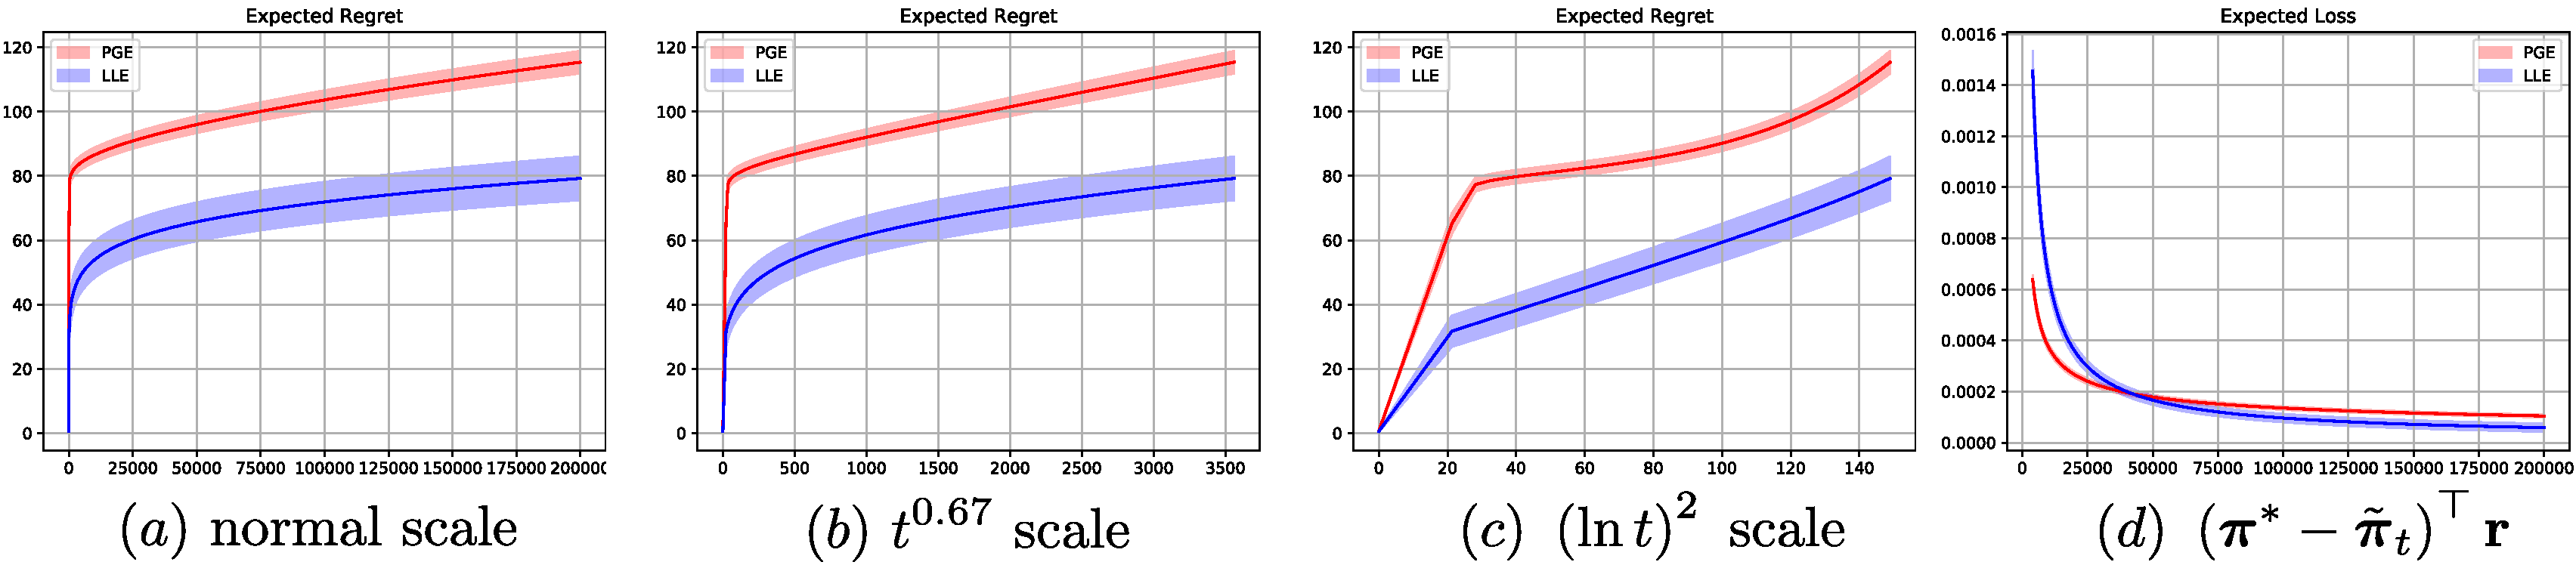
\includegraphics[width=1\linewidth]{comparison_PGE_LLE_regret_scales.pdf}
\caption{The regret of PGE and LLE in different scales, and the expected loss.}
\end{figure*}

We conducted experiments using the proposed PGE and LLE algorithms. The setting is $K = 50$, $m = 5000$, $d = 20$, and $T = 2 \times 10^5$. The true mean reward is uniformly generated $\rvr \in [0.0, 1.0]^K$, then the power $5$ is taken over $\rvr$. The standard deviation of each arm's reward is uniformly randomly generated in $[0.01, 0.05]$. The reward of each sampled action is then generated using a Gaussian distribution with the generated mean and standard deviation.

We repeatedly ran $10$ simulations. In each experiment, the true mean reward and variance are randomly generated. For PGE, $\frac{1}{3} - \beta$ is set to $0.33$, $\sigma = 0.0005$, and $\eta = 0.001$. For LLE, we use $\varepsilon_t = \frac{\ln{t}}{t}$, $\sigma = 0.002$, and $\eta = 0.0005$. At each step $t$, we calculate the expected regret $\sum\limits_{s = 0}^{t - 1}{ ( {\rvpi^*}  - \tilde{\rvpi}_s)^\top \rvr } $ and the latest expected loss $( {\rvpi^*}  - \tilde{\rvpi}_t)^\top \rvr$, where the expectation is taken over the mixed sampling policies in PGE/LLE.

As shown in \cref{fig:regret_loss_scales}, both PGE and LLE obtain expected regrets that are sub-linear in $T$. On the other hand, the expected regret of PGE decays much more slowly than that of LLE, since PGE has a large budget of $t^{\beta - \frac{1}{3}}$ for uniform exploration. We then scale the horizontal axis, to check whether the regret rates in theory are observable. In (b), in scale $t^{0.67}$, the regret of PGE scales almost linearly, indicating its expected regret is about $T^{\frac{2}{3}}$, which is consistent with \cref{thm:policy_gradient_main_result}. Similar results can also be observed for LLE and \cref{thm:logit_learning_main_result}, as shown in (c).


\section{Future Work}
\label{sec:future_work}

Our results are just at the beginning of theoretically understanding the online neural network learning and its combination with reinforcement learning. There are many problems remain open along this line.
\begin{itemize}
    \item \cref{alg:policy_gradient_uniform_exploration} achieves $\tilde{O}(T^{2/3})$ regret. We hypothesize that better rates should be achievable with other strategies. For example, last softmax layer works better with maximum entropy reward \citep{nachum2017bridging}. From this perspective, mirror descent/REINFORCE seem to be natural.
        \item We consider the $\varepsilon$-greedy for exploration. With other type of explorations, like UCB \citep{auer2002finite}, EXP3 \citep{seldin2014one}, and posterior sampling \citep{agrawal2012analysis} can online NN learning and bandit algorithms work well?
    \item Our algorithms use empirical estimation to control functional variation $V_T^f$, which is not scalable for problems in practice. Instead, most practical RL algorithms use sampled reward as an estimation of true reward. However, as mentioned this estimation will have large variation, bringing undesirable learning results. Whether using sampled reward can achieve provable learning results remains open.
    \item In practice, gradient updates always travel a long distance rather than around initialization \citep{liu2018deeptracker}. And usually, practical NNs do not have that much overparametrized scales. Further progresses in the DL theory would be helpful for improving our current analyses of online NN learning and deep reinforcement learning.
    
    \item We investigated the vanilla gradient based algorithms. Combination with other successful RL algorithms including value based and actor critic methods, e.g., DQN \citep{mnih2015human}, A3C \citep{mnih2016asynchronous}, and PCL \citep{nachum2017bridging}, should also be investigated.
    %\item For policy leaning with NN function approximations, there is no known lower bound, although at least the general $\Omega\left(\sqrt{T}\right)$ lower bound holds. We can get some sense from the two parts of the regret in \cref{thm:policy_gradient_main_result}. The NN learning part seems cannot be improved, since this is the best one can obtain under smoothness like properties and gradient upper $\&$ lower bounds. While the other exploration and estimation error part seems still have space to be improved. But whether $\Omega\left(\sqrt{T}\right)$ is achievable is still unknown.
\end{itemize}

\if0
% In the unusual situation where you want a paper to appear in the
% references without citing it in the main text, use \nocite
\nocite{langley00}
\fi

\section{Conclusions}
\label{sec:conclusions}
We established a $\tilde{O}(T^{2/3})$ regret for a straightforward policy based reinforcement learning algorithm under the stochastic multi-armed bandit setting. 
Noting that the main hurdle in our proof is the estimation error $\|\hat{\rvr} - \rvr\|$, we further proposed a value based RL algorithm, Logit Learning with $\varepsilon$-Greedy Exploration (LLE),
and proved that LLE achieves a nearly optimal regret of $O((\ln T)^2)$.
These results can be generalized to many state dependent bandit settings and episodic MDPs, and can be combined with multi-layered neural network function approximators. Our findings are at the starting point of understanding more perspectives and providing theoretical support for deep reinforcement learning techniques. %We also discussed several open problems for future research.


\bibliography{aistats2020}
\bibliographystyle{iclr2020_conference}

\onecolumn
\section{Proofs}

{\bf \cref{lem:equivalence_ment_reinforce}.} Using importance sampling in \cref{alg:erpg_ment_reinforce},
\begin{equation*}
    \nabla{(\rvtheta_t)} = \expectation\limits_{\rho \sim \rvpi_t}{ \left( \rvr_t(\rho) - \tau \log{\rvpi_t(\rho)} \right) \cdot \nabla{ \log{\rvpi_t(\rho)} } }, \quad \forall t \ge 1.
\end{equation*}
\begin{proof}
According to the gradient definition in \cref{alg:erpg_ment_reinforce}, $\forall t \ge 1$,
\begin{equation*}
\begin{split}
    \nabla{(\rvtheta_t)} &= \frac{d \left\{ \rvpi(\rvo_t)^\top \rvr_t - \tau  \rvpi(\rvo_t)^\top \log{\rvpi(\rvo_t)} \right\} }{d \rvtheta_t} \\
    &= \left( \frac{d \rvpi_t}{d \rvo_t} \right)^\top \left( \rvr_t - \tau \rvone - \tau \log{\rvpi_t} \right) \\
    &= \left( \frac{d \rvpi_t}{d \rvtheta_t} \right)^\top \left( \rvr_t - \tau \log{\rvpi_t} \right) \\
    &= \left( \frac{d \rvpi_t}{d \rvtheta_t} \right)^\top \left[ \sum\limits_{i \in [K]}{ \rvpi_t(i) \cdot \rvone_{ \left\{ \frac{\rvr_t(i) - \tau \log{\rvpi_t(i)} }{\rvpi_t(i)} \right\} } } \right] \quad \left( \text{importance sampling} \right) \\
    &= \sum\limits_{i \in [K]}{ \rvpi_t(i) \cdot \left[ \left( \frac{d \rvpi_t}{d \rvtheta_t} \right)^\top \rvone_{ \left\{ \frac{\rvr_t(i) - \tau \log{\rvpi_t(i)} }{\rvpi_t(i)} \right\} } \right] } \\
    &= \sum\limits_{i \in [K]}{ \rvpi_t(i) \cdot \left[ \frac{\rvr_t(i) - \tau  \log{\rvpi_t(i)} }{\rvpi_t(i)} \cdot \frac{d \rvpi_t(i)}{d \rvtheta_t}  \right] } \\
    &= \expectation\limits_{\rho \sim \rvpi_t}{ \left( \rvr_t(\rho) - \tau  \log{\rvpi_t(\rho)} \right) \cdot \nabla{ \log{\rvpi_t(\rho)} } }. \qedhere
\end{split}
\end{equation*}
\end{proof}


{\bf \cref{thm:logit_mean_approximation}.} Let $\rvr_1, \rvr_2, \dots, \rvr_t \in \left[ 0, 1  \right]^K$. Denote $\rvr_{1:t} \triangleq \sum\limits_{i=1}^{t}{\rvr_i}$, and $\hat{\rvr}_t \triangleq \frac{\rvr_{1:t}}{t}$. Consider the following policy gradient update in logit space,
\begin{equation*}
\begin{split}
    \rvo_{t+1} &= \rvo_t + \eta \cdot \nabla(\rvo_t),
\end{split}
\end{equation*}
where $\nabla(\rvo_t) \triangleq \frac{d \left\{ \rvpi(\rvo_t)^\top \rvr_t - \tau \rvpi(\rvo_t)^\top \log{\rvpi(\rvo_t)} \right\} }{d \rvo_t} $ is the policy gradient with respect to $\rvo_t$. If the learning rate $\eta$ at iteration $t$ satisfies
\begin{equation*}
\begin{split}
    \eta \ge \frac{ \frac{1}{t+1} + \frac{1}{(t+1)(t+C)} }{ \frac{1}{K \cdot \exp\left\{ \frac{1}{\tau} \right\} } \cdot \left( 1 - \frac{2 C \sqrt{K}}{\tau t} \right)  } = K \cdot \exp\left\{ \frac{1}{\tau} \right\} \cdot \left( 1 + \frac{1}{t+C} \right) \cdot \frac{t}{\left( t+1\right) \left( t - \frac{2C\sqrt{K}}{\tau} \right)} = O\left( \frac{1}{t} \right),
\end{split}
\end{equation*}
for some constant $C > 0$, then there exists a scalar $c_{t-1} \in \sR$, such that
\begin{equation*}
    \left\| \tau \rvo_{t} - \hat{\rvr}_{t-1} + c_{t-1} \rvone \right\| \le \frac{C \sqrt{K}}{t}, \quad \forall t \ge 1.
\end{equation*}
\begin{proof}
For any policy $\rvpi$, define $\rmH\left( \rvpi \right) \triangleq \Delta \left( \rvpi \right) - \rvpi \rvpi^\top$, where $\Delta \left( \rvpi \right) \in \sR^{K \times K}$ is a diagonal matrix, with $\rvpi$ as its diagonal. First, calculate the policy gradient with respect to logit at step $t$,
\begin{equation*}
\begin{split}
    \nabla(\rvo_t) &\triangleq \frac{d \left\{ \rvpi(\rvo_t)^\top \rvr_t - \tau \rvpi(\rvo_t)^\top \log{\rvpi(\rvo_t)} \right\} }{d \rvo_t} \\
    &= \rmH_t \left( \rvr_t - \tau \rvo_t \right),
\end{split}
\end{equation*}
where $\rmH_t \triangleq \rmH(\rvpi(\rvo_t))$. Next, use induction on $t$. For $t=1$, let $c_0 = 0$,
\begin{equation*}
\begin{split}
    \left\| \tau \rvo_{1} - \hat{\rvr}_0 + c_0 \rvone \right\| = \left\| \rvzero \right\| = 0 \le C \sqrt{K}.
\end{split}
\end{equation*}
Assume $\left\| \tau \rvo_{t} - \hat{\rvr}_{t-1} + c_{t-1} \rvone \right\| \le \frac{C \sqrt{K}}{t}$ for some $t \ge 1$. There  are two different cases of the update.

\textbf{First case:} $\rvr_t - \tau \rvo_t = a_t \rvone$, for some $a_t \in \sR$. This means $\rvo_{t+1} = \rvo_{t}$ because $\rmH_t a_t \rvone = \rvzero$. Let $c_t \triangleq \frac{(t-1)c_{t-1}}{t} +  \frac{a_t}{t}$, we have
\begin{equation*}
\begin{split}
    \left\| \tau \rvo_{t+1} - \hat{\rvr}_t + c_t \rvone \right\| &= \left\| \tau \rvo_{t} - \hat{\rvr}_t + \frac{(t-1)c_{t-1}}{t} \rvone + \frac{a_t}{t} \rvone \right\| \\
    &= \left\| \tau \rvo_{t} - \frac{\rvr_{1:t-1} + \rvr_t}{t-1} \cdot \frac{t-1}{t} + \frac{(t-1)c_{t-1}}{t} \rvone + \frac{a_t}{t} \rvone \right\| \\
    &= \left\| \tau \rvo_{t} - \hat{\rvr}_{t-1} + \frac{\hat{\rvr}_{t-1}}{t} - \frac{\tau \rvo_t + a_t \rvone}{t} + \frac{(t-1)c_{t-1}}{t} \rvone + \frac{a_t}{t} \rvone \right\| \\
    &= \left\| \frac{t-1}{t} \cdot \left( \tau \rvo_{t} - \hat{\rvr}_{t-1} + c_{t-1} \rvone \right) \right\| \\
    &\le \frac{t-1}{t} \cdot \frac{C \sqrt{K}}{t} \\
    &\le \frac{C \sqrt{K}}{t+1}.
\end{split}
\end{equation*}

\textbf{Second case:} $\rvr_t - \tau \rvo_t \not= a_t \rvone$, for any $a_t \in \sR$. Then $\rvo_{t+1} \not= \rvo_t$. By the inductive hypothesis,
\begin{equation*}
\begin{split}
    \left| \tau \rvo_{t}(i) - \hat{\rvr}_{t-1}(i) + c_{t-1} \right| \le \left\| \tau \rvo_{t} - \hat{\rvr}_{t-1} + c_{t-1} \rvone \right\| \le \frac{C \sqrt{K}}{t}, \quad \forall i \in [K].
\end{split}
\end{equation*}
Denote $i_{\min} \triangleq \argmin\limits_{i \in [K]}{\rvo_t(i)} $, $i_{\max} \triangleq \argmax\limits_{i \in [K]}{\rvo_t(i)} $, and $\gF(\rvo_t) \triangleq \log{\sum\limits_{i = 1}^K{\exp\left\{ \rvo_t(i) \right\}} } \le \rvo_t(i_{\max}) + \log{K}$. The smallest probability of $\rvpi_t$ can be lower bounded as
\begin{equation*}
\begin{split}
    \min\limits_{i \in [K]}{\rvpi_t(i)} &= \min\limits_{i \in [K]}{ \exp\left\{ \rvo_t(i) - \gF(\rvo_t) \right\} } \\
    &= \exp\left\{ \min\limits_{i \in [K]}{\rvo_t(i)} - \gF(\rvo_t) \right\} \\
    &\ge \exp\left\{ \rvo_t(i_{\min}) - \rvo_t(i_{\max}) - \log{K} \right\} \\
    &\ge \exp\left\{ \frac{\hat{\rvr}_{t-1}(i_{\min})}{\tau} - \frac{C \sqrt{K}}{\tau t} - \frac{c_{t-1}}{\tau} - \frac{\hat{\rvr}_{t-1}(i_{\max})}{\tau} - \frac{C \sqrt{K}}{\tau t} + \frac{c_{t-1}}{\tau} - \log{K} \right\} \\
    &\ge \exp\left\{ - \frac{1}{\tau} - \log{K} - \frac{2 C \sqrt{K}}{\tau t} \right\} \\
    &= \frac{1}{ K \cdot \exp\left\{ \frac{1}{\tau} \right\} } \cdot \exp\left\{ - \frac{2 C \sqrt{K}}{\tau t} \right\} \\
    &\ge \frac{1}{K \cdot \exp\left\{ \frac{1}{\tau} \right\}} \cdot \left( 1 - \frac{2 C \sqrt{K}}{\tau t} \right).
\end{split}
\end{equation*}
Using the choice of learning rate $\eta$ at step $t$,
\begin{equation*}
\begin{split}
    \eta \cdot \lambda_{\min}^{+}\left\{ \rmH_t \right\} &\ge \eta \cdot \min\limits_{i \in [K]}{\rvpi_t(i)} \\
    &\ge \eta \cdot \frac{1}{K \cdot \exp\left\{ \frac{1}{\tau} \right\}} \cdot \left( 1 - \frac{2 C \sqrt{K}}{\tau t} \right) \\
    &\ge \frac{1}{t+1} + \frac{1}{(t+1)(t+C)}.
\end{split}
\end{equation*}
Let $c_{t} = c_{t-1}$. According to the update,
\begin{equation*}
\begin{split}
    \tau \rvo_{t+1} - \hat{\rvr}_t + c_{t} \rvone &= \tau \rvo_{t} - \hat{\rvr}_{t-1} + c_{t-1} \rvone + \hat{\rvr}_{t-1} - \hat{\rvr}_t - \eta \cdot \rmH_t \left( \tau \rvo_{t} - \hat{\rvr}_{t-1} + c_{t-1} \rvone \right) - \eta \cdot \rmH_t \left( \hat{\rvr}_{t-1} - \rvr_t \right).
\end{split}
\end{equation*}
Denote $\rvdelta_{t} \triangleq \tau \rvo_{t} - \hat{\rvr}_{t-1} + c_{t-1} \rvone$. Note that
\begin{equation*}
\begin{split}
    \hat{\rvr}_{t-1} - \hat{\rvr}_t &= \frac{\rvr_{1:t-1}}{t-1} - \frac{\rvr_{1:t-1} + \rvr_t}{t} = \frac{\rvr_{1:t-1} - (t-1) \cdot \rvr_t }{t(t-1)} = \frac{1}{t} \cdot \left( \hat{\rvr}_{t-1} - \rvr_t \right).
\end{split}
\end{equation*}
We have the following iterative relation,
\begin{equation*}
\begin{split}
    \rvdelta_{t+1} = \left[ \rmI - \eta \cdot \rmH_t \right] \rvdelta_t + \left[ \frac{1}{t} \cdot \rmI - \eta \cdot \rmH_t \right] \left( \hat{\rvr}_{t-1} - \rvr_t \right).
\end{split}
\end{equation*}
By the triangle and H{\" o}lder's inequality, assuming $\rvdelta_t \not= b_t \rvone$ and $\hat{\rvr}_{t-1} - \rvr_t \not= d_t \rvone$ for any $b_t, d_t \in \sR$,
\begin{equation*}
\begin{split}
    \left\| \rvdelta_{t+1} \right\| &\le \lambda_{\max}\left\{ \rmI - \eta \cdot \rmH_t \right\} \cdot \left\| \rvdelta_{t} \right\| + \lambda_{\max}\left\{ \frac{1}{t} \cdot \rmI - \eta \cdot \rmH_t \right\} \cdot \left\| \hat{\rvr}_{t-1} - \rvr_t \right\| \\
    &\le \left( 1 - \eta \cdot \lambda_{\min}^{+}\left\{ \rmH_t \right\} \right) \cdot \left\| \rvdelta_{t} \right\| + \left( \frac{1}{t} - \eta \cdot \lambda_{\min}^{+}\left\{ \rmH_t \right\} \right) \cdot \sqrt{K} \\
    &\le \left( 1 - \eta \cdot \lambda_{\min}^{+}\left\{ \rmH_t \right\} \right) \cdot \frac{C \sqrt{K}}{t} + \left( \frac{1}{t} - \eta \cdot \lambda_{\min}^{+}\left\{ \rmH_t \right\} \right) \cdot \sqrt{K} \\
    &= \frac{C \sqrt{K}}{t} + \frac{\sqrt{K}}{t} - \eta \cdot \lambda_{\min}^{+}\left\{ \rmH_t \right\} \cdot \left( \frac{C \sqrt{K}}{t} + \sqrt{K} \right) \\
    &\le \frac{C \sqrt{K}}{t} + \frac{\sqrt{K}}{t} - \left[ \frac{1}{t+1} + \frac{1}{(t+1)(t+C)} \right] \cdot \left( \frac{C \sqrt{K}}{t} + \sqrt{K} \right) \\
    &= \frac{C \sqrt{K}}{t+1},
\end{split}
\end{equation*}
where $\lambda_{\min}^{+}\left\{ \rmH_t \right\}$ refers to the smallest positive eigenvalue of $\rmH_t$. If either $\rvdelta_t = b_t \rvone$ or $\hat{\rvr}_{t-1} - \rvr_t = d_t \rvone$, for some $b_t, d_t \in \sR$, the result will be similar. If both $\rvdelta_t = b_t \rvone$ and $\hat{\rvr}_{t-1} - \rvr_t = d_t \rvone$, then
\begin{equation*}
\begin{split}
    \tau \rvo_t - \rvr_t &= \tau \rvo_{t} - \hat{\rvr}_{t-1} + c_{t-1} \rvone + \hat{\rvr}_{t-1} - \rvr_t - c_{t-1} \rvone \\
    &= (b_t + d_t - c_{t-1}) \rvone,
\end{split}
\end{equation*}
which reduces to the first case.
\end{proof}

\begin{lem}
Given any $\rvpi \in \Delta$, define $\rmH\left( \rvpi \right) \triangleq \Delta \left( \rvpi \right) - \rvpi \rvpi^\top$. Sorting $\rvpi$ in ascending order,
\begin{equation*}
\begin{split}
    &\quad \rvpi(1) = \rvpi(2) = \cdots = \rvpi(|\gS_1|) \\
    &< \rvpi(|\gS_1|+1) = \rvpi(|\gS_1|+2) = \cdots = \rvpi(|\gS_1| + |\gS_2|) \\
    &\ \ \vdots \\
    &< \rvpi(K - |\gS_k| + 1) = \rvpi(K - |\gS_k| + 2) = \cdots = \rvpi(K),
\end{split}
\end{equation*}
where $\gS_i \triangleq \left\{ \rvpi(|\gS_{<i}| + 1), \rvpi(|\gS_{<i}| + 2), \dots,  \rvpi(|\gS_{<i}| + |\gS_i|) \right\}$, $\forall 1 \le i \le k$, and $|\gS_{<i}| \triangleq \sum\limits_{j < i}{|\gS_j|}$ satisfy \begin{equation*}
\begin{split}
    \bigcup_{i=1}^{k}{\gS_i} &= \left\{ \rvpi(1), \rvpi(2), \dots, \rvpi(K) \right\} \\
    \gS_i \cap \gS_j &= \emptyset, \quad \forall i \not= j.
\end{split}    
\end{equation*}
Then the eigenvalues of $\rmH\left( \rvpi \right)$ are
\begin{equation*}
\begin{split}
    \lambda_{1} &= 0 \\
    \lambda_{2} = \lambda_{3} = \cdots = \lambda_{|\gS_1|} &= \rvpi(|\gS_1|) \\
    \lambda_{|\gS_1| + 1 } &\in \left( \rvpi(|\gS_1|), \rvpi(|\gS_2|) \right) \\
    \lambda_{|\gS_1| + 2} = \lambda_{|\gS_1| + 3} = \cdots = \lambda_{|\gS_1| + |\gS_2|} &= \rvpi(|\gS_2|) \\
    \lambda_{|\gS_1| + |\gS_2| + 1 } &\in \left( \rvpi(|\gS_2|), \rvpi(|\gS_3|) \right) \\
    &\ \ \vdots \\
    \lambda_{K - |\gS_k| +1} &\in \left( \rvpi(K-1), \rvpi(K) \right) \\
    \lambda_{K - |\gS_k| + 2} = \lambda_{K - |\gS_k| + 3} = \cdots = \lambda_{K} &= \rvpi(K).
\end{split}
\end{equation*}
And for any eigenvalue $\lambda$ of $\rmH(\rvpi)$ such that $\lambda \not= \rvpi(i)$, $\forall i \in [K]$, we have
\begin{equation*}
    \sum\limits_{i=1}^{K}{\frac{\rvpi(i)^2}{\rvpi(i) - \lambda}} = 1.
\end{equation*}
\end{lem}
\begin{proof}
Suppose $\lambda$ is an eigenvalue of $\rmH(\rvpi)$ and $\rvv$ is the corresponding eigenvector, i.e.,
\begin{equation*}
    \rmH(\rvpi) \rvv = \left[ \Delta(\rvpi) - \rvpi\rvpi^\top \right] \rvv = \lambda \rvv.
\end{equation*}
It is easy to check that $\rvv = \rvone$ is the eigenvector of $\lambda_0 = 0$. Next, assuming $\lambda \not= 0$, we have
\begin{equation*}
    \rvpi(i) \left( \rvv(i) - \rvpi^\top \rvv \right) = \lambda \rvv(i), \quad \forall i \in [K].
\end{equation*}
Note if $\rvpi^\top \rvv = 0$, we have $\rvpi(i) \rvv(i) = \lambda \rvv(i)$, $\forall i \in [K]$. Since $\rvv \not= \rvzero$, assume $\rvv(j) \not= 0$, then we have $\rvpi(j) = \lambda$. Suppose $\rvpi(j) \in \gS$
\end{proof}



\if0
\begin{table}[h]
\caption{Sample Table Title} \label{sample-table}
\begin{center}
\begin{tabular}{ll}
\textbf{PART}  &\textbf{DESCRIPTION} \\
\hline \\
Dendrite         &Input terminal \\
Axon             &Output terminal \\
Soma             &Cell body (contains cell nucleus) \\
\end{tabular}
\end{center}
\end{table}

\begin{figure}[h]
\vspace{.3in}
\centerline{\fbox{This figure intentionally left non-blank}}
\vspace{.3in}
\caption{Sample Figure Caption}
\end{figure}

\fi

\end{document}
